%============================================================================
% tento soubor pouzijte jako zaklad
% (c) 2008 Michal Bidlo
% E-mail: bidlom AT fit vutbr cz
%============================================================================
% kodovaní: iso-8859-2 (zmena prikazem iconv, recode nebo cstocs)
%----------------------------------------------------------------------------
% zpracování: make, make pdf, make desky, make clean
% připomínky posílejte na e-mail: bidlom AT fit.vutbr.cz
% vim: set syntax=tex encoding=latin2:
%============================================================================
\documentclass[cover]{fitthesis} % odevzdani do wisu - odkazy, na ktere se da klikat
%\documentclass[cover,print]{fitthesis} % pro tisk - na odkazy se neda klikat
%\documentclass[english,print]{fitthesis} % pro tisk - na odkazy se neda klikat
%      \documentclass[english]{fitthesis}
% * Je-li prace psana v anglickem jazyce, je zapotrebi u tridy pouzit
%   parametr english nasledovne:
%      \documentclass[english]{fitthesis}
% * Neprejete-li si vysazet na prvni strane dokumentu desky, zruste
%   parametr cover

% zde zvolime kodovani, ve kterem je napsan text prace
% "latin2" pro iso8859-2 nebo "cp1250" pro windows-1250, "utf8" pro "utf-8"
%\usepackage{ucs}
\usepackage[utf8]{inputenc}
\usepackage[T1, IL2]{fontenc}
\usepackage{url}
\DeclareUrlCommand\url{\def\UrlLeft{<}\def\UrlRight{>} \urlstyle{tt}}

%zde muzeme vlozit vlastni balicky


% =======================================================================
% balíček "hyperref" vytváří klikací odkazy v pdf, pokud tedy použijeme pdflatex
% problém je, že balíček hyperref musí být uveden jako poslední, takže nemůže
% být v šabloně
\ifWis
\ifx\pdfoutput\undefined % nejedeme pod pdflatexem
\else
  \usepackage{color}
  \usepackage[unicode,colorlinks,hyperindex,plainpages=false,pdftex]{hyperref}
  \definecolor{links}{rgb}{0.4,0.5,0}
  \definecolor{anchors}{rgb}{1,0,0}
  \def\AnchorColor{anchors}
  \def\LinkColor{links}
  \def\pdfBorderAttrs{/Border [0 0 0] }  % bez okrajů kolem odkazů
  \pdfcompresslevel=9
\fi
\fi

%Informace o praci/projektu
%---------------------------------------------------------------------------
\projectinfo{
  %Prace
  project=BP,           %typ prace BP/DP
  year=2015,             %rok
  date=\today,           %datum odevzdani
  %Nazev prace
  title.cs=Knihovna pro rychlé zpracování síťových dat,  %nazev prace v cestine
  title.en=Library for Fast Network Traffic Processing, %nazev prace v anglictine
  %Autor
  author=Lukáš Vokráčko,   %jmeno prijmeni autora
  %author.title.p=Bc., %titul pred jmenem (nepovinne)
  %author.title.a=PhD, %titul za jmenem (nepovinne)
  %Ustav
  department=UPSY, % doplnte spravnou zkratku ustavu: UPSY/UIFS/UITS/UPGM
  %Skolitel
  supervisor=Kořenek Jan, %jmeno prijmeni skolitele
  supervisor.title.p=Ing.,   %titul pred jmenem (nepovinne)
  supervisor.title.a=Ph.D.,    %titul za jmenem (nepovinne)
  %Klicova slova, abstrakty, prohlaseni a podekovani je mozne definovat
  %bud pomoci nasledujicich parametru nebo pomoci vyhrazenych maker (viz dale)
  %===========================================================================
  %Klicova slova
  keywords.cs={Klíčová slova v českém jazyce.}, %klicova slova v ceskem jazyce
  keywords.en={Klíčová slova v anglickém jazyce.}, %klicova slova v anglickem jazyce
  %Abstract
  abstract.cs={Výtah (abstrakt) práce v českém jazyce.}, % abstrakt v ceskem jazyce
  abstract.en={Výtah (abstrakt) práce v anglickém jazyce.}, % abstrakt v anglickem jazyce
  %Prohlaseni
  declaration={Prohlašuji, že jsem tuto bakalářskou práci vypracoval samostatně pod vedením pana ...},
  %Podekovani (nepovinne)
  acknowledgment={Zde je možné uvést poděkování vedoucímu práce a těm, kteří poskytli odbornou pomoc.} % nepovinne
}

%Abstrakt (cesky, anglicky)
%\abstract[cs]{Do tohoto odstavce bude zapsán výtah (abstrakt) práce v českém jazyce.}
%\abstract[en]{Do tohoto odstavce bude zapsán výtah (abstrakt) práce v anglickém jazyce.}

%Klicova slova (cesky, anglicky)
%\keywords[cs]{Sem budou zapsána jednotlivá klíčová slova v českém jazyce, oddělená čárkami.}
%\keywords[en]{Sem budou zapsána jednotlivá klíčová slova v anglickém jazyce, oddělená čárkami.}

%Prohlaseni
%\declaration{Prohlašuji, že jsem tuto bakalářskou práci vypracoval samostatně pod vedením pana X...
%Další informace mi poskytli...
%Uvedl jsem všechny literární prameny a publikace, ze kterých jsem čerpal.}

%Podekovani (nepovinne)
%\acknowledgment{V této sekci je možno uvést poděkování vedoucímu práce a těm, kteří poskytli odbornou pomoc
%(externí zadavatel, konzultant, apod.).}

\begin{document}
  % Vysazeni titulnich stran
  % ----------------------------------------------
  \maketitle
  % Obsah
  % ----------------------------------------------
  \tableofcontents

  % Seznam obrazku a tabulek (pokud prace obsahuje velke mnozstvi obrazku, tak se to hodi)
  % \listoffigures
  % \listoftables

  % Text prace
  % ----------------------------------------------
  %=========================================================================

\chapter{Úvod} % #####################################################################################

Žijeme v době, kdy se internet stal nedílnou součástí každodenního života a s internetem už nepracují
pouze klasické počítače, ale do popředí se také dostávají mobilní zařízení, které meziročně
zaznamenávají více než $50\%$ nárůst. Dalším druhem zařízení, jež se začínají připojovat
jsou vestavěné systémy patřící do trendu nazývaného internet věcí.
Rychlostí s jakou přibývají nový uživatelé internetu a zařízení vyžadující přístup k počítačovým sítím
se neustále zvyšují požadavky na rychlost, se kterou data prochází počítačovými
sítěmi a z toho vyplývající požadavky na rychlost zpracování síťového provozu a to zejména na zařízeních
starajících se o řízení internetového provozu na páteřních linkách. Mezi tyto
zařízení lze zařadit směrovače, které řídí datové toky mezi jednotlivými sítěmi,
přepínače starající se o řízení toků dat uvnitř autonomních sítí a
systémy pro detekci (IDS\footnote{Intrusion detection system}) a prevenci (IPS\footnote{Intrusion prevention system})
síťových útoků, které analyzují obsah každého paketu procházejícího sítí.

Páteřní spoje v době psaní této práce dosahují rychlostí v řádech desítek gigabitů
za sekundu a z toho vyplývají požadavky na rychlost zpracování síťových dat. Při těchto rychlostech
jsou tradiční procesory schopny vykonat pouze desítky instrukcí, což nestačí na provedení všech potřebných
operací. Nicméně je důležité, aby stejné rychlosti zpracování dosahovaly všechna zařízení na páteřních spojích,
protože počítačová sít je pouze tak rychlá, jak rychlá je její nejpomalejší část, tzv. úzké hrdlo.

Z těchto vlastností vycházejí požadavky na stále efektivnější algoritmy zpracovávající časově kritické operace.
Časově kritické operace jsou takové operace, jež při zpracování síťového provozu trvají nejdelší dobu a rozbor
těchto operací je součástí této práce. Z těchto operací jsou vybrány a rozvedeny operace
hledání řetězců a regulárních výrazů, analýza a extrakce hlaviček paketů a klasifikace paketů, speciálně pak jednodimenzionální klasifikace dle cílové IP adresy, hledání nejdelšího shodného prefixu.

Přínosem této práce je implementace algoritmů provádějících zmíněných časově kritické operace v podobě knihovny,
která bude využita výzkumnou skupinou ANT na Fakultě Informačních technologií Vysokého učení technického v Brně
pro vytváření bezpečnostních systémů a aplikací.

V kapitole \ref{chapter:theoretical} jsou popsány síťové modely a vrstvy těchto modelů,
nad nimiž jsou operace této knihovny implementovány, dále jsou popsány časově kritické operace prováděné
prvky v počítačových sítích. Kapitola \ref{chapter:api} popisuje návrh veřejného rozhraní vytvořené knihovny
pro operace zmíněné v kapitole \ref{chapter:theoretical}, způsoby použití této knihovny a možnosti rozšíření
o další časově kritické operace. V kapitole \ref{chapter:results} jsou vizualizovány a diskutovány
výsledky, jichž se podařilo dosáhnout v implementaci této knihovny a to na dvou hlavních platformách, Intel a ARM.
Kapitola \ref{chapter:conclusion} shrnuje dosažené výsledky a nastiňuje další možný vývoj této knihovny.

\chapter{Teoretický rozbor}\label{chapter:theoretical} % ###########################################################

Tato kapitola poskytuje teoretické informace, ze kterých vychází tato práce.
V první části je popsán síťový model ISO/OSI a jeho vrstvy důležité z pohledu této práce.
V druhé části jsou pak podrobněji rozebrány jednotlivé časově kritické operace a největší důraz je
kladen na jednodimenzionální klasifikaci paketů, vyhledání nejdelšího shodného prefixu.


\section{Síťové modely}\label{section:models} % #######################################################################
Zpracování dat síťového provozu je rozděleno do několika úrovní. Tyto úrovně jsou popsány síťovými modely.
Základním modelem je ISO/OSI, který slouží pro abstraktní rozdělení operací zpracování síťových dat a využití
našel pouze v akademické sféře. V reálných počítačových sítích pak dominuje model TCP/IP, který má oproti
ISO/OSI modelu menší počet vrstev. Model ISO/OSI je rozdělen na sedm vrstev. V pořadí od nejnižší úrovně to
jsou vrstvy fyzická, linková, síťová, transportní, relační, prezentační a aplikační. Pro tuto práci jsou
podstatné pouze první čtyři vrstvy. Ty jsou detailněji popsány v následující části. Na obrázku \ref{fig:layers} je
znázorněn průchod jednoho datového paketu odeslaného ze stanice A s cílovou adresou stanice B jednotlivými vrstvami modelu ISO/OSI. Jak je z obrázku patrné tak různé druhy síťových zařízení pracují s různými vrstvami.

\begin{figure}[!htbp]
	\centering
	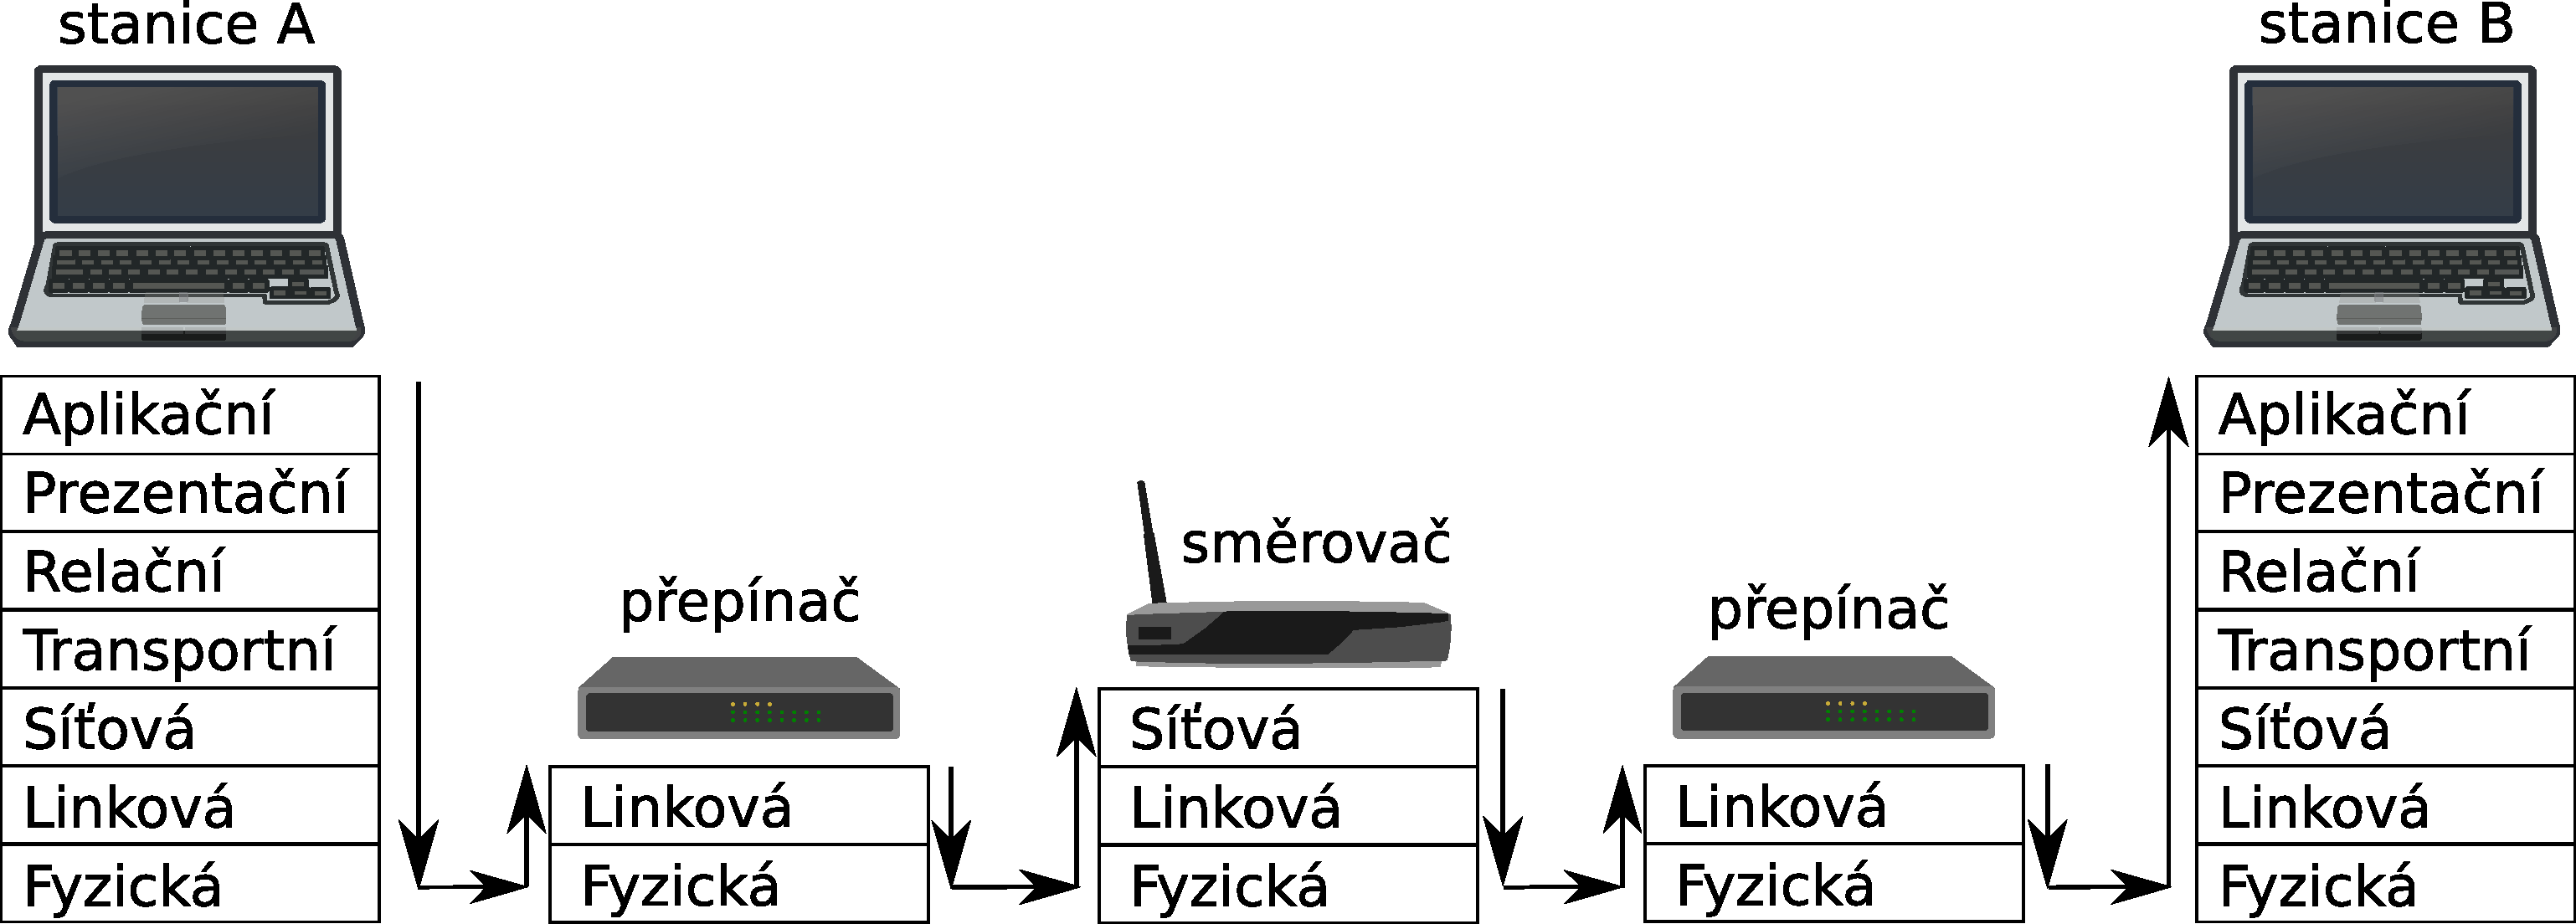
\includegraphics[scale=.25]{fig/layers.pdf}
	\caption{Znázornění průchodu dat počítačovou sítí v modelu ISO/OSI}
    \label{fig:layers}
\end{figure}

\begin{description}
\item[Fyzická vrstva / Vrstva síťového rozhraní]\label{layers:physical} % ##################################
je nejnižší vrstva ISO/OSI modelu a pracuje s daty na úrovni bitů. Stará se o
jejich přenos po přenosovém médiu. Protokoly této vrstvy definují signály reprezentující data,
a tudíž jde o protokoly implementované již v hardware síťových zařízení.

\item[Linková vrstva]\label{layers:link} % ###################################################################
je druhá nejnižší ISO/OSI modelu. Tato vrstva se stará o datovou komunikaci
obecně mezi několika uzly, které jsou přímo spojeny. Spojení může být jak fyzickým vodičem tak i
bezdrátovou technologií. Nejrozšířenější technologií pro fyzické spoje je Ethernet IEEE 802.3 a pro bezdrátové spoje
je to standard IEEE 802.11. Datová jednotka na linkové vrstvě se nazývá rámec a nese v sobě kromě
zapouzdřených dat vyšších vrstev také informace o kontrolním součtu dat a adresování pomocí MAC adres.
MAC adresa je adresa fyzického zařízení, které pracuje na této vrstvě.
Adresování MAC adresou slouží pro identifikaci zařízení, které se nacházejí ve stejné počítačové síti
a za hranici této sítě se již používá IP adresace, která je vysvětlena v následujícím odstavci.
Síťová zařízení pracující na této vrstvě se nazývají přepínače (angl. \textit{switch}).
Úkolem přepínačů je odeslat vstupní data portem, který vede k cílovému zařízení.

\item[Síťová vrstva]\label{layers:network} % ###############################################################
se stará o adresaci zařízení připojených do internetu pomocí síťových adres a o směrování paketů.
Nejrozšířenějším protokolem této vrstvy je protokol IP, jež existuje ve dvou verzích a to IPv4 a IPv6.
Síťová vrstva umožňuje komunikovat zařízením, které nejsou spojeny přímo, ale existuje mezi nimi jedna nebo více cest.
Prvky pracující na této vrstvě jsou nazývány směrovače (angl. \textit{router}) a pracují s datovou strukturou zvanou
datagramy, jež obsahují právě IP adresy jednoznačně určující zdrojové a cílové zařízení. Směrování paketů
je věnována kapitola \ref{section:lpm}

\item[Transportní vrstva]\label{layers:transport} % #########################################################
umožňuje adresovat aplikace zodpovědné za přenášená data. Datová struktura této vrstvy
je nazývána segment. Mezi dominující protokoly patří TCP a UDP. Hlavním rozdílem mezi těmito protokoly
je zaručení spolehlivého doručení a vytváření trvanlivých spojení, které poskytuje pouze TCP.
UDP naopak spolehlivé doručení negarantuje, ale díky tomu je tento protokol jednodušší.
Situace, ve kterých pozitiva jako
nižší režie přebijí zápory je hlavně přenos dat v reálném čase. To je například streamování videa,
přenos hlasu technologie VoIP nebo přenos informací do online her.
Zpracování dat na úrovni transportní vrstvy a všech vyšších vrstev není implementováno na síťových
zařízeních starajících se přenos dat po síti. Jediná zařízení, které implementují zpracování
dat těchto vrstev, jsou koncová zařízení.

\end{description}

\section{Časově kritické operace} % ############################################################################
Pod pojmem časově kritické operace se rozumí takové operace, které zabírají nejvíce výpočetního
času při zpracování jednoho paketu a typicky je nutné provádět je na více síťových zařízeních.
Těmito zařízeními mohou být směrovače, přepínače, firewally a také systémy
oddělené od řízení síťového provozu jako například sondy pouze monitorující síťový provoz nebo analyzátory,
které mohou hledat signatury útoků v datových tocích.

Mezi časově kritické operace rozebrané v této práci patří klasifikace paketů a velký důraz je kladen na
jednodimenzionální klasifikaci dle cílové IP adresy, vyhledávání nejdelšího shodného prefixu.
Tato operace je využívána pro prohledávání směrovací tabulky směrovačů pro určení nejvhodnější cesty jakou
bude paket pokračovat při své cestě k cílovému zařízení.
Další z operací je analýza a extrakce hlaviček paketů, která je využívána v již zmíněné klasifikaci paketů,
kde je nutné z hlavičky paketu extrahovat všechny informace dle kterých bude paket klasifikován.
Dalšími z rozebíraných operací je hledání řetězců a hledání regulárních výrazů.
Poslední dvě zmíněné operace slouží především pro detekci útoků v systémech IDS (z angl. \textit{intrusion detection system})
a pro prevenci útoků v systémech IPS (z angl. \textit{intrusion prevention system}). Jedná se o operace sloužící
pro hloubkové prohledávání paketů (angl. \textit{Deep Packet Inspection}). Toto prohledávání na rozdíl od ostatních operací
pracuje s datovým obsahem paketů a ne jenom s hlavičkami paketu. Z toho vychází časová náročnost,
neboť místo vyhodnocení hlavičky paketu, jež čítá 19 bytů pro IPv4 a 40 bytů pro IPv6 je nutno
projít veškerá data, jejichž velikost se typicky pohybuje v rozmezí $1 - 1500B$.

Informace zde použité vycházejí z publikací \cite{bspl}, \cite{tbm}, \cite{aho}, \cite{gigabit-networking}, \cite{phe-design} a \cite{meduna}.

\subsection{Klasifikace paketů}

Klasifikace paketů je operace rozhodující o dalším zpracování paketu.
Výsledkem klasifikace pak může být rozhodnutí, zda daný paket může projít do
dalšího vyhodnocování nebo zda pochází nebo směřuje do sítě, která není dovolena.
Této klasifikace se využívá například pro povolení pouze určitého rozsahu zdrojových IP adres
pro omezení přístupu do podnikové sítě nebo pro blokování paketů snažících se přistupovat
ke službám, které jsou povoleny pouze pro specifická zařízení.

Data využívané pro klasifikaci se skládají z položek hlavičky paketu, pravidla a priority.
Nejčastěji využívanou klasifikací je klasifikace skládající se z pětice položek IP hlavičky
a to zdrojové adresy, cílové adresy, zdrojového portu, cílového portu a protokolu transportní vrstvy.
Obsahem klasifikačních pravidel pak mohou být přesně specifikované hodnoty, rozsahy nebo prefixy.
Prefixy jsou obecnějším zápisem specifických hodnot i rozsahů, neboť rozsah lze přepsat v nejhorším
případě na $2N - 2$ prefixů \cite{clasification-prefix}, kde $N$ odpovídá počtu bitů reprezentující rozsah. V případě specifické hodnoty je to prefix pouze jeden o bitové délce stejné jako reprezentovaná hodnota.

Klasifikace je prováděna jako vyhledání každé definované položky v množině reprezentující hodnoty
této položky definované v klasifikátoru a poté výběr pravidla s nejvyšší prioritou z kartézského součinu těchto množin.

Tato práce se zabývá pouze jednodimenzionální klasifikací paketů, jež je založena na klasifikaci cílové IP
adresy, hledání nejdelšího shodného prefixu, operace sloužící pro prohledávání směrovacích tabulek směrovačů.

\subsection{Hledání nejdelšího shodného prefixu}\label{section:lpm} % #######################################
Problém hledání nejdelšího shodného prefixu se rozumí jednodimenzionální klasifikace paketů dle
jejich cílové IP adresy, která může být jak verze 4, tak verze 6.
Hledání nejdelšího shodného prefixu je operace, která je prováděna
na síťových prvcích zvaných směrovače. Tyto prvky jsou umístěny na každém rozhraní dvou a více
počítačových sítích. Jejich cílem je nalézt nejvhodnější cestu, kterou směrovat příchozí paket.
Struktura reprezentující uložené směrovací informace se nazývá směrovací tabulka.
Tato tabulka ukládá informace o dostupných sítích (jejich prefixech), délce tohoto prefixu a rozhraní,
kterým se lze do odpovídající sítě dostat. Příklad směrovací tabulky je zobrazen v tabulce \ref{tab:routing-table}

\begin{table}[!htbp]
	\center
    \begin{tabular}{|l|l|l|}
    \hline
    Prefix        & Délka prefixu & Rozhraní \\ \hhline{|=|=|=|}
    147.228.0.0   & 14            & eth0       \\ \hline
    147.228.128.0 & 17            & eth0       \\ \hline
    \end{tabular}
    \caption{Příklad směrovací tabulky}
    \label{tab:routing-table}
\end{table}

S velkým rozmachem počítačových sítí v poslední dekádě dochází k velkému nárůstu směrovacích informací a z toho vycházející nárůst velikosti směrovacích tabulek. Jako jedno z řešení pro zmenšení směrovacích tabulek byl navržen takzvaný supernetting, který agreguje směrovací záznamy
sdílející stejné rozhraní a mající společnou část prefixu do jednoho záznamu.
Pokud vezmeme v úvahu výše uvedenou tabulku tak při použití supernettingu by byly oba záznamy sloučeny
v jeden, který by vypadal takto: $147.228.0.0/14, eth0$.
Tím je dosaženo zmenšení směrovacích tabulek, nicméně i s využitím supernettingu zůstává hledání nejdelšího shodného
prefixu časově kritickou operací.

Prefix ve směrovací tabulce je interně reprezentován jako posloupnost nul a jedniček (binární vyjádření jeho hodnoty) s hvězdičkou na konci která značí, že všechny adresy, jejichž začátek je shodný s částí před hvězdičkou, odpovídají tomuto prefixu.
Jako příklad mějme prefix $A = 1001*$ jež odpovídá adresám začínajícím $1001$, tedy $10010*$ i $10011*$.
Nicméně ve směrovací tabulce může být uložen i prefix B $10010*$, který sdílí první čtyři bity své adresy
s výše uvedeným prefixem $A$ a v případě, že přijde paket začínající hodnotou $10010$ je z pohledu směrování
nutno vyhodnotit prefix B jako nejdelší shodný a poté paket správně směrovat. V případě $10011$ je však nejdelším
shodným prefixem pravidlo A a tudíž nesmí dojít k vyhodnocení prefixu B jako nejdelšího.
Z toho důvodu je nutné ve směrovací tabulce uchovávat i informace o délce prefixu.
Tato informace slouží pro rozhodnutí, jaké pravidlo směrovací tabulky odpovídá nejdelšímu shodnému prefixu.
Délka prefixu může nabývat hodnot $1-32$ pro adresy typu
IPv4 a $1-128$ pro adresy typu IPv6.
Z výše uvedených informací a příkladů vyplývá,
že je nutné rozlišovat, zda existující prefix reprezentuje adresu verze IPv4 nebo IPv6,
jinak by mohlo docházet k vyhodnocení nejdelšího shodného prefixu pro adresu IPv4
jako prefix verze IPv6, což by mělo za následek nevalidní směrování paketů.
Jako příklad může sloužit následující směrovací tabulka, ve které je první pravidlo
verze IPv4 a druhé IPv6. Při vyhledání nejdelšího shodného prefixu v této tabulce by nebylo možné určit jaké pravidlo je to správné.
Pro rozlišení o jaký druh prefixu se jedná je možno použít dva přístupy, rozlišení na úrovni
záznamů směrovacích tabulek nebo rozlišením na úrovni směrovacích tabulek. V této práci je zvoleno rozlišení
na úrovní směrovacích tabulek.

\begin{table}[!htbp]
	\center
    \begin{tabular}{|l|l|l|l|}
    \hline
    Prefix & Délka prefixu & Rozhraní \\ \hhline{|=|=|=|=|}
    $100*$ & 3 & eth0 \\ \hline
    $100*$ & 3 & eth3 \\ \hline
    \end{tabular}
    \caption{Příklad směrovací tabulky}
\end{table}

Pro hledání nejdelšího shodného prefixu existuje velké množství algoritmů, které jsou popsány v \cite{tbm}.
Většina z nich je založena na procházení stromové struktury. Každý algoritmus má jiné paměťové nároky
a dosahuje jiných rychlostí. Z toho důvodu je při výběru vhodného algoritmu nutné
volit kompromis mezi rychlostí a paměťovou náročností.
V případě že jde o implementaci na architektuře FPGA bude důraz pravděpodobně kladen na paměťovou náročnost
a to z důvodu, že tyto čipy mají omezenou kapacitu paměti. Na architekturách vycházejících z x86 je naopak kladen důraz
na rychlost zpracování z důvodu obecných procesorů, které nejsou specializovány na zpracování těchto operací
a dosahují tak delší doby zpracování.

První algoritmus hledání nejdelšího shodného prefixu byl založen na naivním procházení lineárního
seznamu. Doba vyhledávání pomocí tohoto algoritmu byla závislá na počtu uložených prefixů a její
časová složitost byla $O(N)$, což při dnešních rychlostech spojů umožňuje procházet směrovací tabulku
obsahující pouze malý počet záznamů.

Algoritmy rozebrané v této kapitole vycházejí z obecně multibitového stromu,
jež je rozšířením binárního stromu na více než dva potomky.
Těmito algoritmy je binární vyhledávání na délce prefixu a TreeBitmap.
Binární vyhledávání na délce prefixu používá binární strom pro interní reprezentaci směrovacích
informací a pro vyhledávání využívá struktury hašovací tabulky, ve které jsou uloženy všechny existující uzly
binárního stromu.
TreeBitmap je algoritmus založený na multibitovém stromu a vyznačuje se tím,
že pro uložení prefixu využívá zakódované bitmapy a každý uzel stromu může uchovávat informace pro větší počet bitů prefixu, díky čemuž dosahuje menší paměťových nároků.
Dosažené výsledky pro různý počet bitů jsou vizualizovány v kapitole \ref{section:results-lpm}.


\subsubsection{TreeBitmap} % #####################################################################################

Algoritmus TreeBitmap je založen na datové struktuře multibitového stromu, v němž jsou uloženy směrovací informace.
Hlavní myšlenkou je uložení potomků uzlu na jednom paměťovém místě, což znamená, že stačí uchovávat pouze jednu
adresu reprezentující paměťové místo, kde se uzly nacházejí, a index pro určení jaký uzel se má vybrat. Právě
hodnota indexů je zakódovaná do bitmap.
Výhodou tohoto zakódování informací je zmenšení paměťových nároků pro uložení každého uzlu stromové struktury.
Další specifickou vlastností algoritmu TreeBitmap je zpracování několika bitů adresy v jednom kroku.
Počet zpracovaných bitů je nazýván střída a právě velikost střídy určuje počet bitů zakódovaných do jednoho uzlu stromu.

Každý uzel stromové struktury obsahuje dvě bitmapy, interní a externí, které slouží pro zakódování indexů.
Interní bitmapa slouží pro zakódování informací, jaké prefixy se nacházejí v aktuálním uzlu.
Externí bitmapa pak uchovává informace o existujících cestách do nižších vrstev stromové struktury.
Příklad zakódovaných bitmap pro střídu 2 je zobrazen v tabulce \ref{tab:tbm-bitmaps}.
Dalšími položkami uzlu je ukazatel na paměťové místo kde jsou uloženy potomci uzlu a ukazatel na pole obsahující směrovací pravidla, jež odpovídají adresám reprezentovaných tímto uzlem.

\begin{table}
	\center
    \begin{tabular}{|l||c|c|c|c|c|c|c|}
    \hline
    Prefix & $*$ & $0*$ & $1*$ & $00*$ & $01*$ & $10*$ & $11*$ \\ \hhline{|=#=|=|=|=|=|=|=|}
    Interní bitmapa & 0 & 1 & 0 & 0 & 0 & 1 & 1 \\ \hline
    \multicolumn{4}{|l|}{Externí bitmapa} & 1 & 0 & 1 & 0 \\ \hline
    \end{tabular}
    \caption{Příklad bitmap algoritmu TreeBitmap}
    \label{tab:tbm-bitmaps}
\end{table}

Algoritmus vyhledávání spočívá v procházení stromu od kořenu a zjišťování, zda
existuje prefix odpovídající zpracované části adresy. Částí adresy se rozumí N bitů, jež jsou brány postupně
od nejvýznamnějších bitů hledané adresy až po nejméně významné.
Jako první operace hledání nejdelšího shodného prefixu se extrahují bity adresy na pozici odpovídající
aktuální hloubce zanoření ve stromu a provede se operace zjištění, zda je pro část této adresy uloženo
směrovací pravidlo. To je zjištěno z interní bitmapy na pozici, jež odpovídá délce a hodnotě extrahovaných bitů.
Pozice v interní bitmapě je vypočítána jako $2^{N} - 1 + x$, kde $N$ reprezentuje hodnotu střídy a $x$
je dekadickou reprezentací extrahovaných bitů.
Pokud je na této pozici
hodnota "1", je uloženo pravidlo na indexu spočítatelným jako \texttt{ones(bitmap, position)} v poli pravidel.
Toto pravidlo pak reprezentuje dočasný nejlepší výsledek. Pokud je na vypočítané
pozici v interní bitmapě hodnota "0" je opakován výpočet pozice s hodnotou $N$ sníženou o jedna a bitovou hodnotou
oříznutou o nejméně významný bit. Tato operace se opakuje tak dlouho, dokud není nalezena pozice
s hodnotou "1"
nebo dokud není N nulové. Jako druhá operace je provedeno hledání následovníků ve stromové struktuře
reprezentující specifičtější prefixy. To je provedeno jako zjištění přítomnosti hodnoty "1" v externí
bitmapě na pozici, jejíž hodnota je dekadickou reprezentací extrahovaných bitů. V případě přítomnosti
"1" na této pozici je proveden přechod do další úrovně stromové struktury a celý postup se opakuje.
Pokud je na této pozici hodnota "0" je vyhledávání ukončeno a jako výsledek je navrácena hodnota
dočasného nejlepšího výsledku, která odpovídá pravidlu jež patří k nejdelšímu shodnému nalezenému
prefixu. Celý algoritmus je popsán pseudokódem v algoritmu \ref{alg:treebitmap}.

Pro výpočet indexu do polí obsahující pravidla a následovníky se používá funkce
\texttt{ones(bitmap, position)}, jež
spočítá počet bitů s hodnotou "1" v dané bitmapě a to od pozice 0 do pozice \texttt{position}.

Jeden uzel stromu TreeBitmap je vizualizován na obrázku \ref{fig:tbm-node}. Uzly zbarvené černě
jsou uzly, pro které je definováno směrovací pravidlo.

\begin{figure}[!htbp]
    \centering
    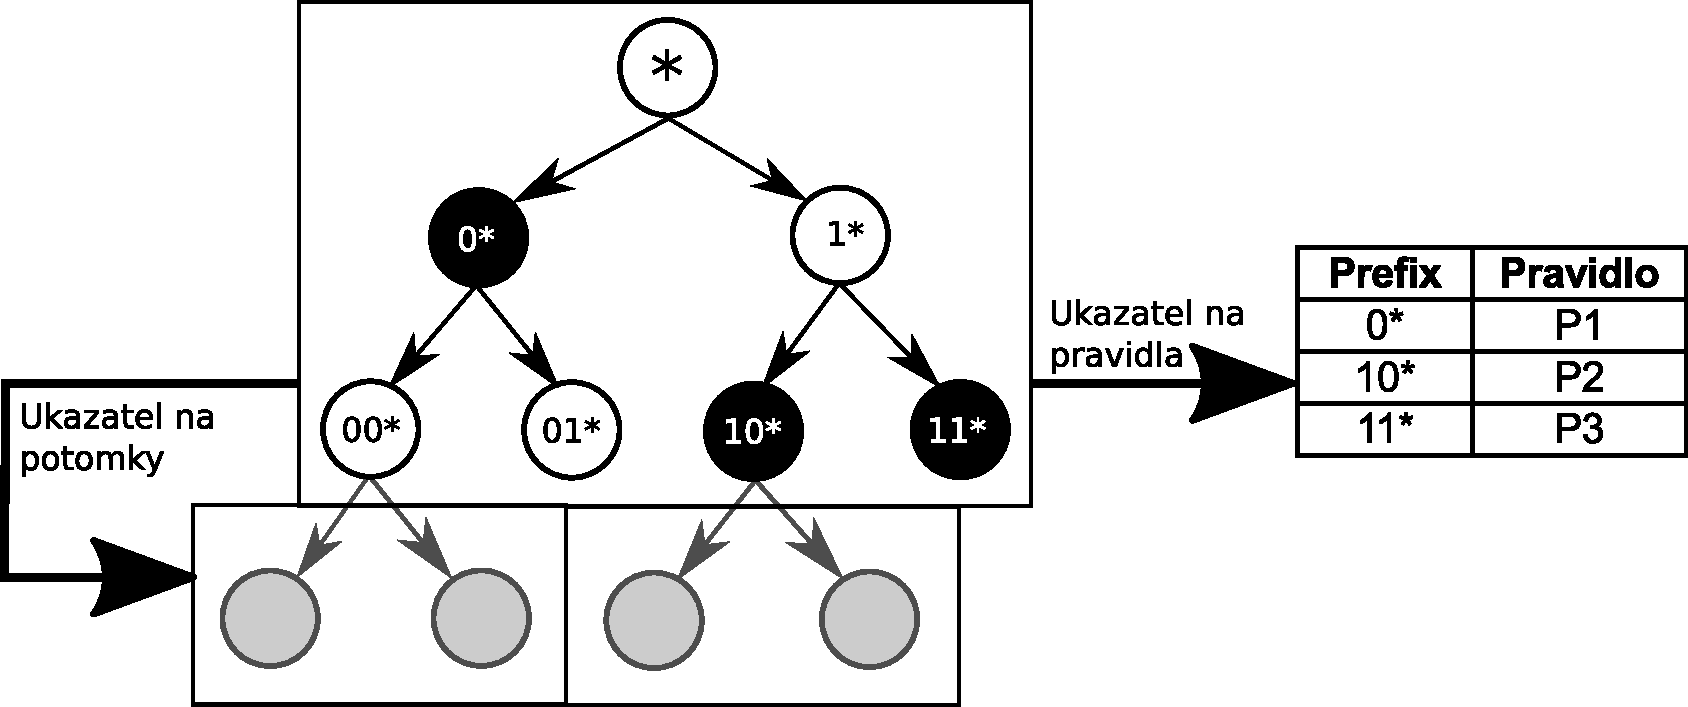
\includegraphics[scale=.55]{fig/tbm.pdf}
    \caption{Jeden uzel algoritmu TreeBitmap}
    \label{fig:tbm-node}
\end{figure}

\begin{algorithm}[H]
	\KwData{tbm-root, ip}
	\KwResult{routing rule}
	node $\leftarrow$ tbm-root\;
	longest-match-node $\leftarrow$ tbm-root\;
	longest-match-index $\leftarrow$ 0\;
	position $\leftarrow$ 0\;
	\Repeat{BIT(parent.external, bits)}
	{
		bits $\leftarrow$ get-stride-bits(ip, position)\;
		position $\leftarrow$ position + STRIDE\;


		\If{internal-index(node.internal, bits)}
		{
			longest-match-node = node\;
			longest-match-index = internal-index(node.internal, bits)\;
		}

		index $\leftarrow$ ones(node.external, bits)\;
		parent $\leftarrow$ node\;
		node $\leftarrow$ node.external[index]\;
	}
	\Return longest-match-node.rule[logest-match-index]\;
	\caption{Hledání nejdelšího shodného prefixu algoritmem TreeBitmap}
    \label{alg:treebitmap}
\end{algorithm}

\subsubsection{Binární vyhledávání na délce prefixu} % ###########################################################

Algoritmus binárního vyhledávání na délce prefixu vychází z jednobitového binárního stromu a přidává
operaci propagování listů (angl. \textit{leaf-pushing}) a zavádí efektivnější prohledávání založené na hašovací
tabulce. Hodnota klíče uzlu v obecném binárním stromu není přímo zanesena do uzlu jako jedna z jeho položek,
ale odpovídá cestě stromem od kořene k aktuálnímu uzlu.
Struktura uzlu je rozšířena o položky prefix, délka prefixu a typ uzlu.
Typy uzlu jsou dva a to interní uzel mající právě dva potomky a uzel reprezentující pravidlo.
Oproti binárnímu stromu používá tento algoritmus i hašovací tabulku, do které jsou zaneseny všechny uzly
stromu a jako hodnota pro hašovací funkci je použita hodnota prefixu v daném uzlu.


Operace propagace listů je operace zaručující, že existují právě dva následovníci uzlu (typ internal) nebo neexistuje žádný (typ prefix).
Pokud dojde ke stavu, že existuje právě jeden následovník uzlu je operací propagování uzlů
vytvořen i druhý uzel a je do něj zaneseno pravidlo, jež obsahuje nadřazený uzel.
Ukázku stromu před operací propagace listů je možno vidět na obrázku \ref{bspl-not-pushed}
a po provedení této operace na obrázku \ref{bspl-pushed}.

\begin{figure}[!htbp]
    \begin{floatrow}
        \ffigbox{
        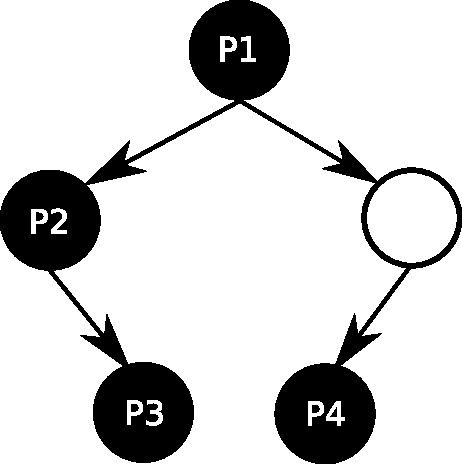
\includegraphics[scale = 0.5]{fig/bspl-not-pushed.pdf}}
            {\caption{Strom před leaf-pushingem}\label{bspl-not-pushed}}
        \ffigbox{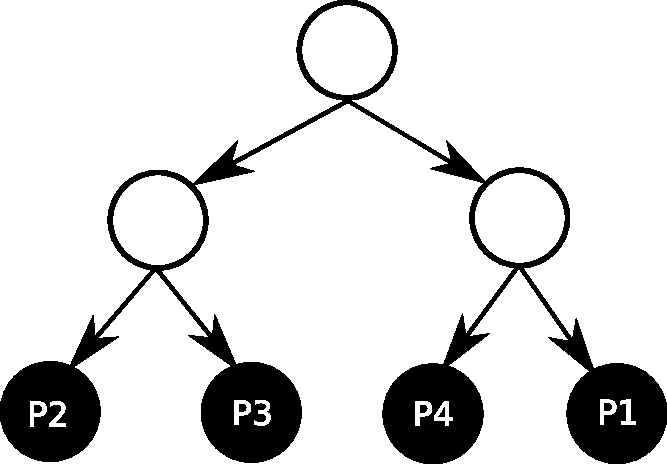
\includegraphics[scale = 0.5]{fig/bspl-pushed.pdf}}
            {\caption{Strom po provedení leaf-pushingu}\label{bspl-pushed}}
    \end{floatrow}
\end{figure}


Vyhledávání nejdelšího shodného prefixu v hašovací tabulce se skládá z následujících kroků.
Jako první je provedeno hledání celé IP adresy, tedy všech 32 bitů v případě IPv4 nebo 128 bitů pro IPv6.
Pokud je vyhledání úspěšné a nalezený prvek je typu prefix, pak je pravidlo tohoto uzlu navráceno
jako nejdelší shodný prefix. V případě kdy nalezený prvek je typu internal nebo není nalezen žádný prvek dojde ke změně délky prefixu o hodnotu $2^{N - krok + 1}$, kde $N = 5$ pro IPv4 a $N = 7$ pro IPv6.
V případě nalezení uzlu typu internal je délka adresy zvýšena o tuto hodnotu.
Pokud není nalezen žádný prvek tak je délka adresy snížena o tuto hodnotu.
Tento postup se opakuje dokud není nalezen prvek typu prefix nebo je hodnota změny prefixu rovna nule.
Algoritmus zapsaný pseudokódem je popsán v \ref{alg:bspl}.
Příklad vyhledávání konkrétního prefixu je popsán v tabulce \ref{tab:bspl-example} ve směrovací tabulce \ref{tab:bspl-table-example}.

\begin{table}[!htbp]
	\center
    \begin{tabular}{|l|l|l|}
    \hline
    Prefix        & Délka prefixu & Pravidlo \\ \hhline{|=|=|=|}
    147.228.0.0   & 14            & P1       \\ \hline
    147.228.128.0 & 17            & P2       \\ \hline
    \end{tabular}
    \label{tab:bspl-table-example}
    \caption{Příklad směrovací tabulky}
\end{table}

\begin{table}[!htbp]
	\center
    \begin{tabular}{|l|r|l|r|l|}
    \hline
    Prefix & Délka & Uzel & Změna délky & Výsledek \\ \hhline{|=|=|=|=|=|}
    147.228.128.54 & 32 & Nenalezen & -16 &  \\ \hline
    147.228.0.0 & 16 & Interní & +8 &  \\ \hline
    147.228.128.0 & 24 & Nenalezen & -4 &  \\ \hline
    147.228.128.0 & 20 & Nenalezen & -2 &  \\ \hline
    147.228.128.0 & 18 & Nenalezen & -1 &  \\ \hline
    147.228.128.0 & 17 & Prefix & 0 & P2 \\ \hline
    \end{tabular}
    \label{tab:bspl-example}
    \caption{Příklad vyhledání nejdelšího shodného prefixu}
\end{table}

Operace vyhledání nejdelšího prefixu při využití binárního vyhledávání na délce prefixu má časovou
složitost při ideální hašovací funkci $\log_2{N}$, kde \texttt{N} je počet bitů adresy. V případě IPv4 adresy je to 32 bitů a pro IPv6
adresu je to 128 bitů. Z principu algoritmu vyplývá, že nejhorší výsledky z časového hlediska bude dosahovat
při shodě prefixu, který byl zadán s lichou délkou. V takovém případě bude nutné projít všemi kroky.
Počet kroků v případě IPv4 bude 5 a v případě IPv6 adresy to pak bude 7.
Zde je vidět že i v případě čtyřikrát delší adresy se počet kroků pro vyhledání prefixu zvedne pouze o dva,
což neplatí pro algoritmus TreeBitmap, který musí projít v nejhorším případě až čtyřikrát více
uzlů aby nalezl odpovídající prefix.
\cite{bspl}

\begin{algorithm}
	\KwData{bspl-root, hash-table, ip, ip-length}
	\KwResult{routing rule}
	prefix-length $\leftarrow$ ip-length\;
	prefix-change $\leftarrow$ ip-length\;
	\Repeat{prefix-change $>$ 0}
	{
		bits $\leftarrow$ get-prefix-bits(ip, prefix-length)\;
		item $\leftarrow$ hash-table.get(bits)\;
		prefix-change $\leftarrow$ prefix-change $\gg$ 1\;

		\lIf{item == NULL}{prefix-length $\leftarrow$ prefix-length - prefix-change}
		\lElseIf{item.type == PREFIX}{prefix-length $\leftarrow$ prefix-length + prefix-change}
		\lElse{break}
	}
	\lIf{item == NULL}{\Return bspl-root.default-rule}
	\caption{Hledání nejdelšího shodného prefixu algoritmem Binary search on prefix length}
\end{algorithm}

\subsection{Hledání řetězců} % ###################################################################

Jednu z častých operací při zpracování síťového provozu je hledání řetězců, jež je využíváno pro detekci
signatur útoků na počítačové sítě, detekci malware a blokování dat obsahujících zakázaná klíčová slova.
Hledání řetězců je ověřování, zda se jedno a více definovaných klíčových slov vyskytuje ve vstupních
datech. V případě počítačových sítí se vstupními daty rozumí datových obsah paketů.

Pokud se oprostíme od počítačových sítí, tak dalším využitím hledání řetězců může být
vyhledávání klíčových slov v textových dokumentech, což bylo důvodem pro vznik
algoritmu autorů Aho a Corasickové, kteří tímto způsobem zrychlili prohledávání
textových dokumentů až $5\times$. Alternativou k algoritmu Aho-Corasick může být požadován
algoritmus autorů Rabin–Karp \cite{rabin-karp}, který má ovšem průměrnou časovou složitost $O(m+n)$,
zatímco pro Aho-Corasick je tato složitost nejhorší možná. Algoritmem vycházejícím z Aho-Corasick
a Boyer–Moore \cite{boyer-moore}
je Commentz-Walter \cite{walter}, jehož časová složitost však v nejhorším případě dosahuje $O(m*n)$.
Algoritmem na nějž se soustředí část této práce je právě Aho-Corasick.
Tento algoritmus používá pro zjištění shody s podřetězcem konceptu konečného automatu.

Konstrukce konečného automatu reprezentujícího klíčová slova je prováděna postupně a to tím způsobem,
že je v automatu hledán již existující prefix vkládaného klíčového slova. Od výsledku tohoto hledání
se pak vychází v dalších krocích, jež jsou následující:

\begin{description}
    \item[Vstup  $\leq$ Existující] v tomto případě je pouze vloženo další pravidlo k danému uzlu.
    \item[Vstup $>$ Existující] v tomto případě je rozšířena již existující cesta a do koncového
    uzlu této cesty je přiřazeno odpovídající pravidlo.
\end{description}

Po dokončení operace přidávání klíčových slov je provedeno generování tzv. \textit{failure} přechodů.
\textit{Failure} přechod je mapováním dalšího přechodu, který je proveden v případě, že pro vstupní symbol neexistuje
přechod z aktuálního stavu. \textit{Failure} přechod pak reprezentuje prefix klíčových slov,
který je podřetězcem aktuálně procházeného klíčového slova.
Generování \textit{failure} cesty je definováno iterativně a to následujícím způsobem:

Pro počáteční uzel je failure cesta definována jako přechod do sebe sama.
Pro každý uzel v úrovni 1 je failure cesta definována jako přechod do počátečního stavu.
Pro každou další úroveň je možné \textit{failure} přechod zjistit z validních přechodů stavu v nižších úrovních.

Příkladem procházení automatu a hledání slov může sloužit následující příklad reprezentovaný tabulkami
\ref{tab:pm-keywords} a \ref{tab:pm-match} při vstupních datech \textit{ship}.
Symbol $[]$ reprezentuje počáteční stav a $[xyz]$ reprezentuje posloupnost stavů odpovídající cestě od
počátečního symbolu do aktuální cesty.

\begin{table}[!htbp]
    \center
    \begin{tabular}{|l|l|}
    \hline
    Klíčové slovo & Pravidlo \\ \hhline{|=|=|}
    she & 1  \\ \hline
    hi & 2 \\ \hline
    \end{tabular}
    \caption{Klíčová slova}
    \label{tab:pm-keywords}
\end{table}

Automat reprezentující tyto klíčová slova je zobrazen na obrázku \ref{fig:ac}.
Plnou čarou jsou znázorněny možné přechody, přerušovanou čarou \textit{failure} přechody a zelenou
je znázorněn průchod automatem v pro vstupní data \texttt{ship}.

\begin{figure}[!htbp]
    \centering
    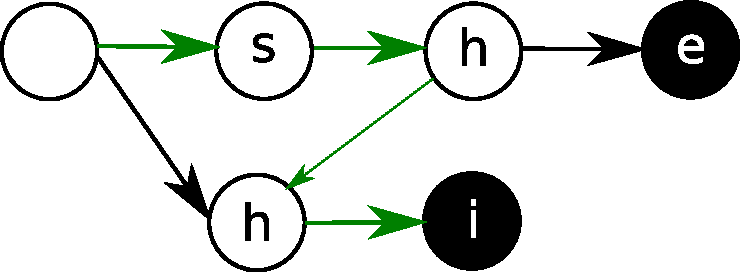
\includegraphics[scale=.55]{fig/ac.pdf}
    \caption{Automat obsahující klíčová slova \texttt{she} a \texttt{hi}}
    \label{fig:ac}
\end{figure}

\begin{table}[!htbp]
	\center
    \begin{tabular}{|l|l|l|}
    \hline
    Aktuální symbol & Akce automatu & Výsledek \\ \hhline{|=|=|=|}
    s & [] $\overset{s}{\rightarrow}$ [s] &  \\ \hline
    h & [s] $\overset{h}{\rightarrow}$ [sh] & \\ \hline
    i & $\nexists$ [sh] $\overset{i}{\rightarrow}$ [shi], [sh] $\overset{\epsilon}{\rightarrow}$ [h], [h] $\overset{i}{\rightarrow}$ [hi] & \texttt{hi} \\ \hline
    p & $\nexists$ [hi] $\overset{p}{\rightarrow}$ [hip], [hi] $\overset{\epsilon}{\rightarrow}$ [], [] $\overset{p}{\rightarrow}$ [] &  \\ \hline
    \end{tabular}
    \caption{Prohledávání algoritmem Aho-Corasick}
	\label{tab:pm-match}
\end{table}


Algoritmus procházení vstupních dat je popsán pseudokódem v \ref{alg:aho} a vychází z \cite{aho}.

\begin{algorithm}[!htbp]
	\KwData{start-state, text}
	\KwResult{keyword}
	state = start-state\;
	\For{position $\leftarrow$ 0 \KwTo text.length}
	{
		\lWhile{goto(state, text[position]) == FAIL}{state $\leftarrow$ state.failure}
		\lIf{state.isMatch}{\Return state.keyword}
	}
	\Return NOT-MATCH\;
	\caption{Algoritmus procházení textu a hledání podřetězců}
    \label{alg:aho}
\end{algorithm}

\subsection{Hledání regulárních výrazů}\label{sec:regex} % ############################################

Hledání regulárních výrazů je, podobně jako hledání řetězců, operace sloužící pro detekci signatur
síťových útoků a detekci škodlivého software v obsahu datových paketů v systémech IDS a IPS.
Algoritmy pro hledání regulárních výrazů v rámci této práce jsou založeny na transformaci
regulárních výrazů na konečné automaty.
V této práci jsou rozebrány deterministické a nedeterministické konečné automaty.

Než se dostaneme k popisu jednotlivých druhů konečných automatů je potřeba definovat co jsou to regulární
výrazy a jaké operace je s nimi možno provádět.

Nechť $r$ a $s$ jsou regulární výrazy značící jazyky $L_R$ a $L_S$.
Regulární výrazy nad abecedou $\Sigma$ a jazyky které značí jsou definovány následovně

\begin{itemize}
    \item{$\emptyset$ je RV značící prázdnou množinu (prázdný jazyk)}
    \item{$\epsilon$ je RV značící jazyk ${\epsilon}$}
    \item{$a$, kde $a \in \Sigma$ je RV značící jazyk ${a}$}
    \item{$r.s$ je RV značící jazyk $L = L_R L_S$}
    \item{$r+s$ je RV značící jazyk $L = L_S \cup L_S$}
    \item{$r*$ je RV značící jazyk $L = L_{R*}$}
\end{itemize}

Časová složitost pro jednotlivé varianty je následující

\begin{itemize}
\item{nedeterministické konečné automaty $O(n*m)$}
\item{deterministické konečné automaty $O(n)$}
\end{itemize}

Průchod deterministický konečným automatem je možné zpracovat právě jeden znak vstupu v
každé iteraci. Algoritmus se podívá, zda existuje přechod pro aktuální znak na vstupu z aktuálního stavu,
a pokud existuje tak je proveden přechod. V případě, že takový přechod neexistuje, tak je nastaven
aktuální stav na počáteční stav konečného automatu a operace je provedena znovu.
Algoritmus procházení deterministickým konečným automatem je popsán v \ref{alg:dfa},
procházení nedeterministického automatu je popsán v \ref{alg:nfa}.

\begin{algorithm}
    \KwData{root - startovní stav konečného automatu, input - vstupní data, length - délka vstupních dat}
    \KwResult{vyhovuje/nevyhovuje}
    position $\leftarrow 0$
    state $\leftarrow$ root
    \While{length > position}
    {
        symbol $\leftarrow$ input[position]\;
        states.push(root)\;

        \While{state $\leftarrow$ states.pop()}
        {
            \lIf{state->key[symbol]}{states-new.push(state->next[symbol])}
            \lIf{state->next[symbol].accepting} {\Return state->next[symbol].rule}
        }

        swap(states, states-new)\;
        position $\leftarrow position + 1$\;
    }
    \caption{Algoritmus procházení pro deterministický konečný automat}
    \label{alg:dfa}
\end{algorithm}

\begin{algorithm}
    \KwData{root - startovní stav konečného automatu, input - vstupní data, length - délka vstupních dat}
    \KwResult{vyhovuje/nevyhovuje}
    position $\leftarrow 0$
    state $\leftarrow$ root
    \While{length > position}
    {
        symbol $\leftarrow$ input[position]\;
        states.push(root)\;

        \While{state $\leftarrow$ states.pop()}
        {
            \lFor{ i $\leftarrow$ 0 \KwTo i $<$ state.epsilon\_count}{states.push(state.epsilon[i])}
            \lIf{state->key[symbol]}{states-new.push(state->next[symbol])}
            \lIf{state->next[symbol].accepting} {\Return state->next[symbol].rule}
        }

        swap(states, states-new)\;
        position $\leftarrow position + 1$\;
    }
    \caption{Algoritmus procházení pro nedeterministický konečný automat}
    \label{alg:nfa}
\end{algorithm}

\subsection{Analýza a extrakce hlaviček paketů} % ###################################################

Extrakce hlaviček paketů je operace prováděná na každém síťovém zařízení,
neboť právě na základě hodnot položek hlavičky paketu je prováděno rozhodnutí,
jak má být paket zpracován.
V případě hledání nejdelšího shodného prefixu je potřeba nejprve provést extrakci
cílové adresy a až poté je možné zahájit vyhledávání cesty, kterou bude paket směrován.
Z toho vyplývá přímá závislost rychlosti všech operací pracujících s položkami hlaviček na linkové, síťové a
transportní vrstvě.

Tato operace je celkem komplexní a to z důvodu různé délky jednotlivých hlaviček na vrstvách
linkové, síťové a transportní v závislosti na použitém protokolu na dané vrstvě.
Vstupem operace analýza a extrakce hlaviček paketů je datový paket a výstupem je
množina hodnot, jež byly cílem analýzy a extrakce.

Analýzu a extrakci hlaviček lze provádět jak na úrovni softwarového řešení tak i na úrovní hardware,
jak předvedli autoři v \cite{phe}.

Operace je rozdělena na dva kroky. Prvním krokem je lokalizace požadované hlavičky ve vstupních datech
a druhým je pak extrakce této hodnoty.

Jedním ze způsobů jak extrahovat hlavičky paketů je použití orientovaných acyklických grafů,
kde vrcholy reprezentují typy hlaviček a hrany reprezentují posloupnost hlaviček.
Parsovací graf je převeden na konečný automat.

Operace je možné rozdělit na dvě paralelní zpracování,
kdy v prvním zpracování bude identifikován typ hlavičky a v druhé pak bude provedena extrakce
této hodnoty v závislosti na typu hlavičky a informací, kde se daná položka v hlavičce nachází.

\chapter{Návrh API knihovny}\label{chapter:api} % #################################################################

Cílem návrhu API knihovny \texttt{fastnet} je vhodně zapouzdřit implementované operace a to takovým způsobem,
aby je bylo možné používat bez znalosti využívaných algoritmů. Dalším cílem návrhu je připravit API tak,
aby bylo možné rozšiřovat množinu algoritmů implementující dané operace při zachování
současného API. Je navrženo API pro operace klasifikace paketů \ref{api:pc}, hledání nejdelšího shodného prefixu
\ref{api:lpm}, hledání řetězců \ref{api:pm}, hledání regulárních výrazů \ref{api:regex} a analýzu a
extrakci hlaviček paketů. V kapitole \ref{api:extension} je rozebrána možnost rozšíření této knihovny o další operace a v kapitole \ref{api:usage} je popsáno jakým způsobem je možné sestavit celou knihovnu nebo její jednotlivé
části.

Každá operace umožňuje pracovat s více datovými strukturami reprezentující
data dané operace. Toho je dosaženo explicitním uváděním kořenu místo jeho implicitního uložení
uvnitř knihovny. To byl také jeden z požadavků při návrhu API. Kořenový prvek je
explicitně předáván do funkcí provádějící jednotlivé operace. Jedinou výjimkou
jsou inicializační funkce, které právě vytvářejí kořenovou strukturu pro další použití.

Knihovna \texttt{fastnet} je navržena jako množina menších knihoven, kde každá knihovna implementuje
jednu operaci používanou při zpracování síťového provozu.
Tímto návrhem je dosaženo snadné rozšiřitelnosti o další operace,
jako například extrakce informací z hlaviček paketů a klasifikaci paketů.
Další výhodou tohoto rozdělení je možnost snadno vytvořit a používat jednotlivé knihovny samostatně nebo v různých kombinacích nezahrnující všechny operace.
To se může hodit pro zařízení, která mají velmi limitované paměťové úložiště a jejich účelem
je řešit pouze část ze zmíněných operací.

Veřejné rozhraní celé knihovny se skládá z veřejných rozhraní jednotlivých knihoven.
Tyto rozhraní jsou popsány v následujících kapitolách.

Pro knihovnu je navržena struktura hlavičkových souborů pro jednotlivé knihovny.
Jako výchozí hlavičkový soubor je použit \texttt{types.h},
který obsahuje definice datových struktur pro všechny algoritmy v knihovně, které musí být
viditelné i z veřejného rozhraní. Dalším souborem je \texttt{types-precompiled.h},
který je generován z \texttt{types.h} při překladu když se vybírá používaný algoritmus.
Soubor \texttt{common.h} je hlavičkový soubor společný pro všechny algoritmy v knihovně a \texttt{<algorithm>.h}
pak obsahuje deklarace specifické pro právě jeden konkrétní algoritmus.
Soubor \texttt{<sublib.h>} je pak hlavičkový soubor, který tvoří veřejné rozhraní ke knihovním funkcím.
Závislost jednotlivých souborů je znázorněna na obrázku \ref{fig:header-dependecies}.

\begin{figure}[!htbp]
    \centering
    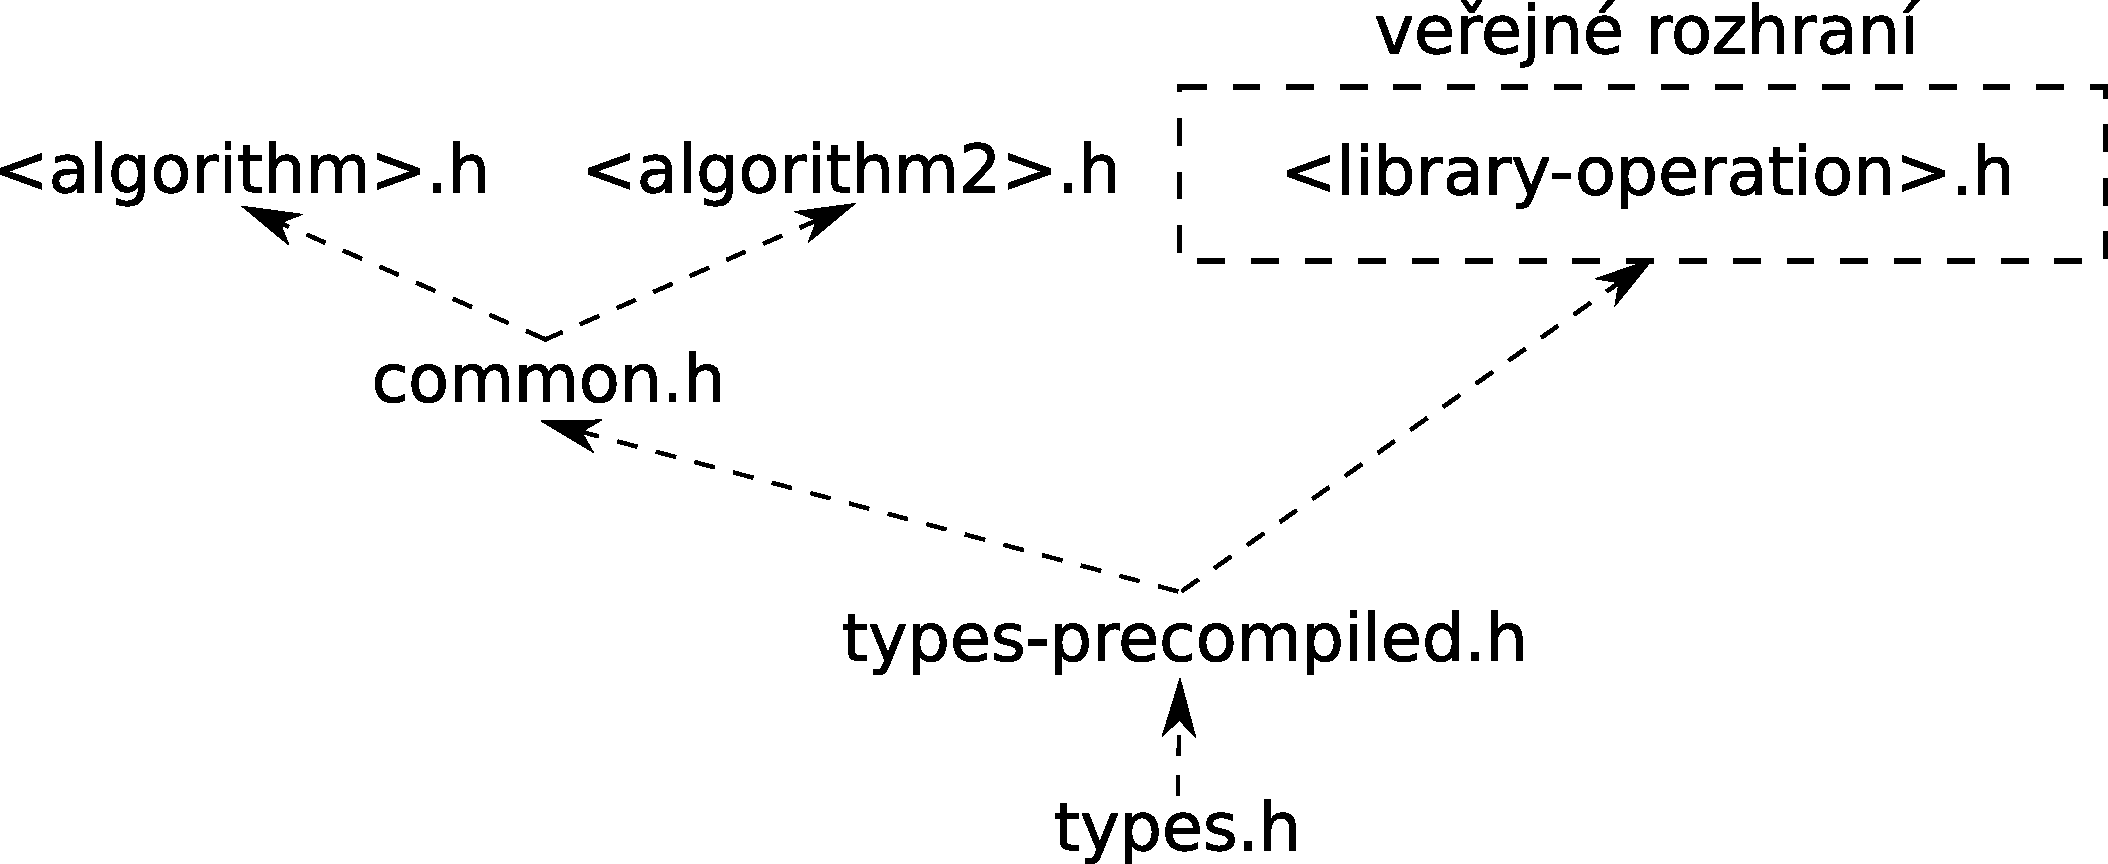
\includegraphics[scale=.25]{fig/header-dependencies.pdf}
    \caption{Diagram závislostí hlavičkových souborů}
    \label{fig:header-dependecies}
\end{figure}


\section{Klasifikace paketů}\label{api:pc} % #######################################################

Pro klasifikaci paketů jsou navrženy čtyři základní funkce a jedna datová struktura.
Tato struktura je nazvána \texttt{set} a obsahuje položky \texttt{rule} pro uložení pravidla,
které odpovídá kombinaci ostatních položek, \texttt{dst} pro uložení cílové IP adresy,
\texttt{src} pro uložení zdrojové adresy, \texttt{protocol} pro uložení typu transportního protokolu,
tedy TCP nebo UDP a \texttt{port} pro uložení cílového portu.
Důvod proč jsou vybrány pouze tyto položky je to, že tato operace není implementována
a tyto položky jsou při klasifikaci používány nejčastěji.

Funkce pro práci se strukturou pro klasifikaci paketů jsou: \texttt{init} pro inicializaci
vyhledávacích struktur, \texttt{add} pro přidání klasifikačního pravidla, \texttt{update}
pro aktualizaci odpovídajícího pravidla, \texttt{remove} pro smazání odpovídajícího pravidla
a nakonec \texttt{destroy} pro uvolnění veškeré paměti zabírané strukturami pro provádění klasifikace
paketů.

Všechny zmíněné funkce a jedna datové struktura jsou navrženy ve dvou verzích a to pro IPv4 a IPv6.
Tyto funkce se od sebe liší pouze prefixem, kde pro IPv4 je použit prefix \texttt{pc\_} a pro
IPv6 pak \texttt{pc6\_}. Důvodem, proč jsou jednotlivé funkce a struktura rozděleny tímto
způsobem ,je odlišná velikost adres a nutnost rozlišovat pro jako verzi IP protokolu se klasifikace provádí,
neboť prefixy adres se mohou shodovat pro obě verze IP, ale mohou reprezentovat jiné adresy.

Všechny funkce vyjma \texttt{init} očekávají jako první argument strukturu typu \texttt{root},
která obsahuje veškeré informace o klasifikačních pravidlech. Jako u ostatních operací
je tato struktura uváděna explicitně a to umožňuje vytvářet více klasifikátorů v jednom programu.

Přesnou specifikaci rozhraní je možné nalézt v přiloženém CD ve složce \texttt{/lib/src/pc/pc.h}

\section{Vyhledání nejdelšího shodného prefixu}\label{api:lpm} %########################################

Pro operaci vyhledání nejdelšího shodného prefixu jsou připraveny funkce
\texttt{init}, \texttt{add}, \texttt{update}, \texttt{remove} a \texttt{destroy}.
Jako datové struktury jsou navrženy struktury pro uložení každého uzlu datového stromu.
Pro binární vyhledávání na délce prefixu to je struktura \texttt{\_bspl\_node} a pro
algoritmus TreeBitmap \texttt{\_tbm\_node}.

Funkce \texttt{init} slouží pro vytvoření kořenového uzlu datových struktur a
nastavení výchozího pravidla, které je vybráno, pokud není nalezen žádný odpovídající prefix.
Návratovou hodnotou této funkce je ukazatel na kořen datové struktury, jež je parametrem
všech ostatní funkcí provádějící operace v rámci vyhledání nejdelšího shodného prefixu.
Funkce \texttt{add} slouží pro přidání prefixu a pravidla odpovídajícímu tomuto prefixu.
Funkce \texttt{update} slouží pro aktualizaci pravidla daného prefixu.
Funkce \texttt{remove} odstraňuje zvolený prefix z vyhledávací struktury.
Funkce \texttt{destroy} slouží pro uvolnění paměti alokované všemi výše zmíněnými funkcemi
a po provedení této funkce již není možné provádět další operace nad danou strukturou.

Funkce pro vložení, smazání a aktualizaci pravidel a prefixů také obsahují parametr
prefix, který je buď IPv4 nebo IPv6 adresa. Dalším parametrem těchto funkcí je délka prefixu,
aby bylo možné odlišit jednotlivé prefixy od sebe.

Funkce pro vložení prefixu pracuje pouze s jedním prefixem a je prováděna okamžitě.
Tento návrh vychází z předpokladu, že knihovna bude používána i v prostředí s dynamickými routovacími
protokoly jako například RIP, OSPF nebo BGP, které při změně směrovacích informací v případě BGP
zasílají aktualizace s novými informacemi na všechny sousední směrovače nebo jsou tyto změny
zasílány periodicky v případě protokolu RIP.

Hašovací funkce je v této implementaci použita Jenkins \cite{jenkins}. Volba hašovací funkce
může mít vliv na rychlost vyhledávání. To je patrné z principu hašovací tabulky, kde se
kolizní záznamy uchovávají v lineárním seznamu a v případě kdy by hašovací funkce generovala
stejné hodnoty pro všechny vstupní hodnoty by bylo vyhledávání omezeno na procházení
lineárního seznamu se složitostí v nejhorším případě $O(log_2{N}*M)$, kde $M$ odpovídá počtu záznamů uložených ve směrovací tabulce a $N$ velikosti IP adresy, tedy 32 nebo 128 bitů
namísto $O(\log_2{N})$, kde N reprezentuje délku IP adresy.

Použitý algoritmus lze volit při sestavení knihovny pro vyhledání nejdelšího shodného prefixu
zapsáním následujícího příkazu \texttt{make ALG=<alg>}, kde hodnota \texttt{<alg>} může nabývat
hodnot \texttt{tbm} pro volbu TreeBitmap a \texttt{bspl} pro binární vyhledávání na délce prefixu.
V případě sestavování celé knihovny je možné zapsat \texttt{make LPM=<alg>} v příslušném adresáři.

Při volbě algoritmu TreeBitmap je pak volitelný parametr \texttt{STRIDE=<N>}, jež určuje velikost
střídy. Tuto volbu je možné použít v obou příkazech.

Přesnou specifikaci rozhraní je možné nalézt v přiloženém CD ve složce \texttt{/lib/src/lpm/lpm.h}
Specifikaci datových struktur lze nalézt v soubor \texttt{/lib/src/lpm/types.h}


\section{Hledání řetězců}\label{api:pm} % ####################################################################

Pro hledání řetězců je navrženo několik datových struktur, mezi které patří
struktura pro uložení právě jednoho stavu konečného automatu \texttt{\_ac\_state},
struktura reprezentující jeden konečný automat \texttt{pm\_root} a struktura \texttt{pm\_keyword}
pro uložení klíčového slova, jeho délky a jemu odpovídající pravidlo.


Pro hledání řetězců jsou podobně jako pro vyhledání nejdelšího shodného prefixu navrženy a implementovány
následující funkce.

\begin{itemize}
    \item{\texttt{pm\_init} pro inicializaci datových struktur}
    \item{\texttt{pm\_match} pro hledání prvního klíčové slova vyskytujícího se ve vstupních datech}
    \item{\texttt{pm\_match\_next} pro hledání dalších klíčových slov}
    \item{\texttt{pm\_add} pro vložení množiny klíčových slov}
    \item{\texttt{pm\_update} pro změnu pravidla odpovídající danému klíčovému slovu}
    \item{\texttt{pm\_remove} pro smazání klíčového slova}
    \item{\texttt{pm\_destroy} pro uvolnění veškeré paměti jež byla alokována}
\end{itemize}

Všechny výše zmíněné funkce vyjma \texttt{pm\_init} a \texttt{pm\_match\_next} očekávají jako první parametr strukturu typu \texttt{pm\_root},
která je základním prvkem pro vyhledávání a právě do této struktury
jsou uložena všechna klíčová slova a jejich pravidla.

Hledání řetězců funkcí \texttt{pm\_match} skončí svůj průchod konečný automatem v momentě nálezu první shody
s libovolným řetězcem zadaným při volání \texttt{pm\_add}.
V případě, že není nalezena žádná shoda
s definovanými klíčovými slovy v řetězci je vrácen výsledek \texttt{false}.

Čtvrtým parametrem funkce \texttt{pm\_match} může být hodnota \texttt{NULL} nebo odkaz na datovou strukturu
\texttt{pm\_result}. V případě \texttt{NULL} argumentu již nelze procházet textem a hledat další shody.
Pokud je zadán odkaz na existující strukturu \texttt{pm\_result} je možné procházet celým textem a ukládat
všechny nalezené shody s klíčovými slovy funkcí \texttt{pm\_match\_next}.

Jednotlivé položky struktury \texttt{pm\_result} pro veřejné použití jsou

\begin{itemize}
    \item{\texttt{rule} - pole obsahující všechny nalezená klíčová slova}
    \item{\texttt{count} - počet nalezených klíčových slov}
    \item{\texttt{position} - pozice kde bylo nalezen výskyt klíčového slova}
\end{itemize}

Pro práci se strukturou \texttt{pm\_result} jsou v navrženy a implementovány následující operace:

\begin{itemize}
    \item{\texttt{pm\_result\_init} pro vytvoření této struktury}
    \item{\texttt{pm\_result\_destroy} pro uvolnění paměti alokované pro tuto strukturu}
\end{itemize}


Funkce \texttt{pm\_add} očekává jako druhý parametr pole struktur \texttt{pm\_keyword}, kde každá struktura
obsahuje položky vstupního klíčové slova v binární podobě, délku tohoto slova a pravidlo odpovídající tomuto slovu, oproti kterým se budou porovnávat vstupní data. Důvodem pro tento návrh je časově náročná funkce generování
\textit{failure} přechodů, které umožňují detekovat kratší klíčové slovo i v případě, že již je
zahájeno porovnávání delšího slova jak je možno vidět na následujícím příkladu. Tabulka \ref{tab:ac:substr}
obsahuje definovaná klíčová slova a obrázek \ref{fig:ac:substr} znázorňuje odpovídající konečný automat.

\begin{table}[!htbp]
    \center
    \begin{tabular}{|l|l|}
    \hline
    Klíčové slovo & Pravidlo \\ \hhline{|=|=|}
    she & 1  \\ \hline
    he & 2 \\ \hline
    \end{tabular}
    \caption{Klíčová slova}
    \label{tab:ac:substr}
\end{table}

\begin{figure}[!htbp]
    \centering
    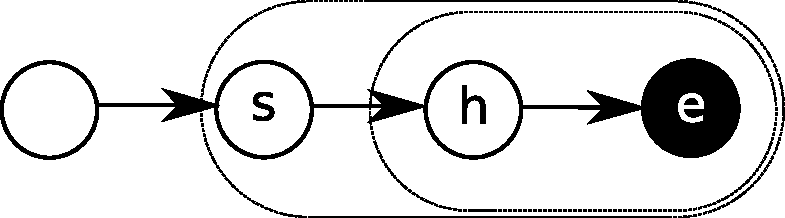
\includegraphics[scale=0.7]{fig/ac-substr.pdf}
    \caption{Konečný automat reprezentující \ref{tab:ac:substr}}
    \label{fig:ac:substr}
\end{figure}


Přesnou specifikaci rozhraní je možné nalézt v přiloženém CD ve složce \texttt{/lib/src/pm/pm.h}
Specifikaci datových struktur lze nalézt v soubor \texttt{/lib/src/pm/types.h}

\section{Hledání regulárních výrazů}\label{api:regex}  % ##########################################################

Rozhraní pro hledání regulárních výrazů navržené a implementované v knihovně \texttt{fastnet:regex}
rozšiřuje množinu operací prováděných s regulárnícmi výrazy zmíněných v \ref{sec:regex} o následující zápisy operací.

\begin{itemize}
    \item{$[abc]$ je výčet znaků, které se na vstupu mohou vyskytnout a automat je v aktuální stavu dokáže zpracovat. Je to zkrácený tvar zápisu $(a|b|c)$}
    \item{$a+$ je definováno jako $1..N$ opakování}
    \item{$a?$ je definováno jako $0..1$ opakování}
\end{itemize}


Pro hledání regulárních výrazů jsou navrženy a implementovány dva způsoby hledání, a to
deterministický \texttt{dfa} a nedeterministický konečný automat \texttt{nfa}.
Z toho důvodu jsou odlišeny všechny funkce dle typu konečného automatu, který je použit.
Pro použití deterministického konečného automatu je to \texttt{dfa} a pro nedeterministický
je to \texttt{nfa}.

Navrženy jsou následující funkce

\begin{itemize}
    \item{\texttt{regex\_<type>\_construct} pro vytvoření regulárního výrazu}
    \item{\texttt{regex\_<type>\_match} pro hledání regulárního výrazu ve vstupních datech}
    \item{\texttt{regex\_<type>\_destroy} a uvolnění paměti zabrané regulárním výrazem}
\end{itemize}
% REGEXDFA =================================================================================

Pokud se v definici regulárního výrazu vyskytuje jeden z řídících znaků regulárních výrazů
je nutno tento znak escapovat, to znamená přidat před něj zpětné lomítko.
Zpětné lomítko samotné se pak zapíše jako dvě zpětná lomítka.

Pro vytvoření regulárních výrazů je podobně jako u hledání řetězců
použita pomocná struktura \texttt{regex\_pattern}, která je předávána do funkce \texttt{regex\_<type>\_construct}
a jež obsahuje pole regulárních výrazů, z nichž se má vytvořit jeden konečný automat.
Výsledný konečný automat, ať už deterministický nebo nedeterministický, je výsledek spojení jednotlivých
konečných automatů pro každý regulární výraz. Tím je umožněna detekce několika
regulární výrazů v jednom průchodu vstupními daty i s přesnou identifikací jaký regulární
výraz byl ve vstupních datech nalezen.

Důvodem proč jsou navrženy obě možnosti pro hledání regulárních výrazů je až teoreticky exponenciální nárůst
počtu stavů deterministického konečného automatu, což může být ve specifických případech nežádoucí a je vhodnější
vyměnit rychlost deterministického konečného automatu za menší paměťové nároky.

Přesnou specifikaci rozhraní je možné nalézt v přiloženém CD v souboru \texttt{/lib/src/regex/regex.h}
Specifikaci datových struktur lze nalézt v soubor \texttt{/lib/src/regex/types.h}

\section{Analýza a extrakce hlaviček paketů}\label{api:phe} %#####################################################

Pro tuto operaci byla navržena jedna funkce a jedna struktura.
Touto strukturou je \texttt{phe\_item}, jež je typu \texttt{union}, jehož položky
se vzájemně překrývají. Důvodem pro tento návrh je ten, že každá položka hlavičky paketů obsahuje právě jednu hodnotu.

Navrženou funkcí je funkce \texttt{phe\_get}, jež jako první parametr očekává
vstupní data, jako druhý délku těchto dat, jako třetí ukazatel na pole \texttt{phe\_item},
kam se budou ukládat jednotlivé extrahované hodnoty.

Funkce dokáže zpracovat variabilní počet argumentů.
Hodnotami pro variabilní argumenty jsou hodnoty typu \texttt{enum}, kde každá hodnot odpovídá
právě jedné položce hlavičky paketu a její číselná hodnota odpovídá počtu bytů
od začátku datové struktury paketu.

Pro efektivnější zpracování je vhodné volit pořadí těchto parametrů stejné jako je jejich reálná
posloupnost ve struktuře paketu.

Některé základní položky využívané při klasifikaci paketů a jejich vzdálenosti od počátku hlavičky
jsou uvedeny v tabulce \ref{tab:phe}

\begin{table}[!htbp]
	\center
    \begin{tabular}{|l|l|l|}
    \hline
    Význam & Název & offset \\ \hhline{|=|=|=|}
    Verze & IP\_VERSION & 0 \\ \hline
    Zdrojová IP adresa pro IPv4 & IP\_SRC & 12 \\ \hline
    Cílová IP adresa pro IPv4 & IP\_DST & 16 \\ \hline
    Cílový port pro IPv4 & PORT\_DST & 22 \\ \hline
    Protokol pro IPv4 & PROTO & 8 \\ \hline
    \end{tabular}
	\caption{Položky IP paketu a jejich pojmenování pro extrakci a analýzu}
    \label{tab:phe}
\end{table}

Přesnou specifikaci rozhraní je možné nalézt v přiloženém CD ve složce \texttt{/lib/src/phe/phe.h}


\section{Použití knihovny}\label{api:usage} % #######################################################################
Celou knihovnu je možné sestavit příkazem \texttt{make all} v hlavním adresáři knihovny.
Při provedení tohoto příkazu bude celá knihovna sestavena s definovaným NDEBUG, což má za následek vypuštění všech
volání funkce assert, která slouží pro ověřování správné funkčnosti.

Dalšími Cíly pro program \texttt{make} jsou

\begin{itemize}
	\item{\texttt{test} - spustí automatické testování všech částí knihovny}
	\item{\texttt{bech} - spustí benchmarky všech částí knihovny}
	\item{\texttt{doc} - vygeneruje programovou dokumentaci ke všem částem knihovny}
	\item{\texttt{clean} - smaže všechny soubory vytvořené překladem}
\end{itemize}

Knihovny reprezentující jednotlivé operace je možné sestavit příkazem \texttt{make}
v odpovídajícím adresáři. Pro překlad s debugovacími informacemi je možno využít cíl sestavení
\texttt{make lib}.

\section{Rozšíření knihovny}\label{api:extension} % ############################################

Pro rozšíření knihovny je nutné přidat knihovnu implementující danou operaci
do adresáře \texttt{lib/src} a upravit příslušný soubor \texttt{Makefile} v daném adresáři.
Dále je vhodné vytvořit testovací program a sadu testů, kterou je možné automatizovaně spouštět a vyhodnocovat.
Tyto soubory pak umístit do adresáře \texttt{lib/test/<operace>}.
Další vhodnou součástí knihovny operace je benchmark pro vyhodnocení rychlosti jednotlivých
implementací dané operace.



\chapter{Výsledky}\label{chapter:results} % ##########################################################################
Tato kapitola shrnuje a vizualizuje dosažené výsledky při implementaci jednotlivých knihoven.
Benchmarky pro architekturu Intel proběhly na operačním systému Archlinux \footnote{https://www.archlinux.org/} s procesorem Intel(R) Core(TM) i3-2310M CPU @ 2.10GHz.

\section{Hledání nejdelšího shodného prefixu}\label{section:results-lpm} % ####################################################################

Hledání nejdelšího shodného prefixu bylo testováno na celkem pěti vstupních sadách dat, které
se liší počtem záznamů směrovací tabulky. Data byla převzata z volně dostupných dat RIPE\footnote{https://www.ripe.net/}.
Počet záznamů směrovacích tabulek, verze IP adres a délky prefixů jsou popsány v tabulce \ref{tab:lpm-input}.
Dosažené výsledky pro jednotlivé sady dat jsou vizualizovány na obrázcích \ref{fig:lpm-ipv4} pro sady IPv4 a
\ref{fig:lpm-ipv6} pro sady IPv6.

\begin{table}[!htbp]
	\center
    \begin{tabular}{|l|l|l|l|}
    \hline
    Počet adres & Nejkratší prefix & Nejdelší prefix & Verze IP \\ \hhline{|=|=|=|=|}
    $1000$ & 13 & 31 & IPv4 \\ \hline
    $10000$ & 8 & 32 & IPv4 \\ \hline
    $100000$ & 8 & 32 & IPv4 \\ \hline
    $1000$ & 23 & 128 & IPv6 \\ \hline
    $10000$ & 19 & 128 & IPv6 \\ \hline
    \end{tabular}
	\caption{Směrovací tabulky pro testování}
    \label{tab:lpm-input}
\end{table}

Vyhledávání bylo prováděno oproti $1000$ IP adresám odpovídající verze. Tyto adresy byly vybrány
ze záznamů směrovacích tabulek použitých pro testy.

\begin{figure}[H]
	\centering
	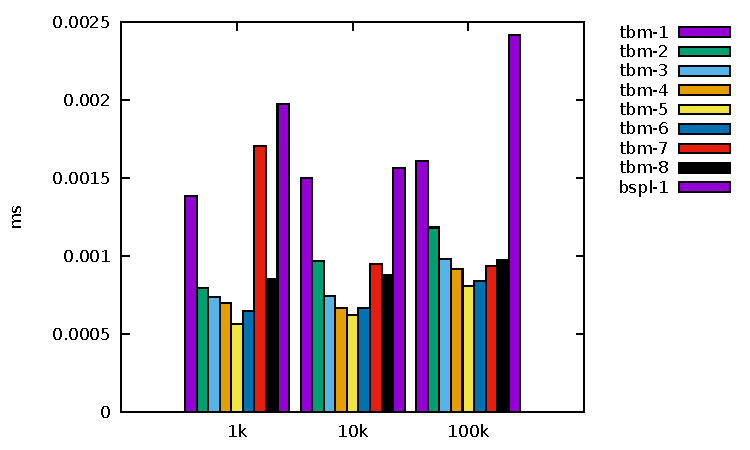
\includegraphics[scale=1]{fig/lpm-ipv4.pdf}
	\caption{Benchmark pro IPv4}
    \label{fig:lpm-ipv4}
\end{figure}

Benchmark byl proveden pro algoritmy TreeBitmap (v grafu označeno jako \texttt{tbm-střída}) ve velikostích střídy $1-8$ a pro binární vyhledávání na délce prefixu (v grafu označeno jako \texttt{bspl-1}).
Jak je možno vyčíst z uvedených grafů, tak nejlepších výsledků bylo dosaženo pro TreeBitmap s velikostí
střídy nastavenou na $5$ bitů a to jak pro IPv4 a $6$ bitů pro IPv6.

\begin{figure}[!htbp]
	\centering
	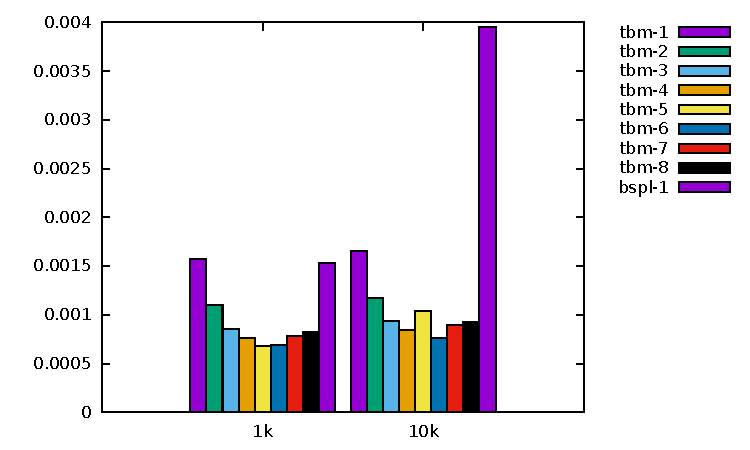
\includegraphics[scale=1]{fig/lpm-ipv6.pdf}
	\caption{Benchmark pro IPv6}
    \label{fig:lpm-ipv6}
\end{figure}

Pro testování algoritmu Binary search on prefix length byla zvolena velikost hašovací tabulky
stejná jako počet záznamů směrovací tabulky pro zvolenou sadu dat. Tento přístup byl zvolen z důvodu významného vlivu
velikosti hašovací tabulky na rychlost samotného vyhledávání.
V případě nastavení velikosti hašovací tabulky na $100$ prvků byl algoritmus vyhledávání pomalejší $400\times$
při použití směrovací tabulky obsahující $100 000$ záznamů.


Dalším důležitým faktorem pro efektivnost implementace je velikost datových struktur, která je
závislá na velikosti střídy pro algoritmus TreeBitmap a také na počtu směrovacích pravidel.
Velikost struktury v závislosti na počtu směrovacích pravidel je ovlivněna následujícím způsobem.
Do 256 záznamů zabírá pravidlo pouze $1B$, do 65536 záznamů pak $2B$ a pro více než 65536 pak celé $4B$ pro uložení právě jednoho pravidla. Rozdíl mezi uložení $65536$ adres a $65537$ adres pak bude činit
$200KB$. Velikost uzlů stromu pro zvolené algoritmy v závislosti na počtu záznamů směrovací tabulky
je popsán v tabulce \ref{tab:lpm-input}.

\begin{table}[!htbp]
	\center
    \begin{tabular}{|l|l|l|l|l|}
    \hline
    & & \multicolumn{3}{l|}{Velikost pro počet směrovacích pravidel} \\ \hline
    Algoritmus & Velikost střídy & $< 256$ & $< 65536$ & $\geq 65536$\\ \hhline{|=|=|=|=|=|}
    TBM & 1 & 24 & 25 & 28 \\ \hline
    TBM & 2 & 24 & 25 & 28\\ \hline
    TBM & 3 & 24 & 25 & 28\\ \hline
    TBM & 4 & 24 & 25 & 28\\ \hline
    TBM & 5 & 32 & 33 & 36\\ \hline
    TBM & 6 & 40 & 41 & 44\\ \hline
    TBM & 7 & 64 & 65 & 68\\ \hline
    TBM & 8 & 112 & 113 & 116\\ \hline
    BSPL & --- & 48 & 49 & 52\\ \hline
    \end{tabular}
	\caption{Velikosti datových struktur v závislosti na počtu směrovacích pravidel a velikosti střídy}
    \label{tab:lpm-input}
\end{table}

Jak je možné vyčíst z výše uvedené tabulky, tak i přestože nejrychlejší implementací pro IPv4 je TreeBitmap se střídou 5, tak v případě omezené paměti by bylo vhodnější zvolit kompromis mezi rychlostí a paměťovou náročností v podobě
TreeBitmap s velikostí střídy 4, který dosahuje nejmneší možné velikosti datové struktury a zároveň nejlepších výsledků pro danou velikost datové struktury.

\section{Hledání řetězců} % #####################################################################################
Testování efektity implementace hledání řetězců bylo provedeno na dvou vstupních testovacích sadách,
kde první sada \texttt{fallbacks} obsahuje slova s výskytem stejných písmen, tudíž při tvorbě konečného automatu bude
docházet ke generování \textit{failure} přechodů, jež budou poté procházeny. Druhá testovací sada \texttt{no-fallbacks}
obsahuje slova, která neobsahují stejná písmena. Výsledky dosažené pro jednotlivé testovací sady jsou
vizualizovány v grafu \ref{fig:pm}. Testování probíhalo na datových paketech odchycených z komunikace osobního počítače. Testovací sady obsahují klíčová slova používaná v protokolu HTTP.

\begin{figure}[!htbp]
	\centering
	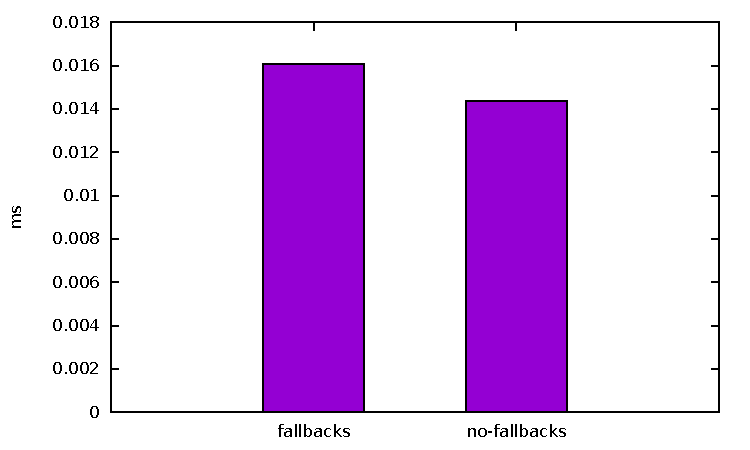
\includegraphics[scale=0.7]{fig/pm.pdf}
	\caption{Benchmark pro knihovnu pm}
    \label{fig:pm}
\end{figure}

Jak je možné vyčíst z grafu tak sada obsahující \textit{failure} přechody dosahuje mírně horších výsledků,
což je způsobeno delším zpracování znaku, pro který neexistuje validní přechod v aktuálním stavu konečného automatu.

Velikost každého stavu konečného automatu je v této implementaci $48B$
a podobně jako hledání nejdelšího shodného prefixu je závislá na počtu vložených pravidel.

\section{Hledání regulárních výrazů} % ###############################################################################

Jak je vidět na v grafu \ref{fig:regex} tak hledání regulárních výrazů pomocí deterministického
konečného automatu je řádově pomalejší. Toto zpomalení je způsobené nutností procházení $\epsilon$-přechodů.
Procházení založené na deterministickém konečném automatu tímto problémem netrpí,
neboť při zpracování každého vstupního symbolu dojde k přechodu do dalšího stavu v případě
vstupního symbolu, který se může vyskytnou v aktuálním stavu automatu nebo do počátečního stavu
pokud vstupní symbol nejde zpracovat v rámci regulárního výrazu.

Dopsat na jakých datech byl benchmark proveden

\begin{figure}[!htbp]
	\centering
	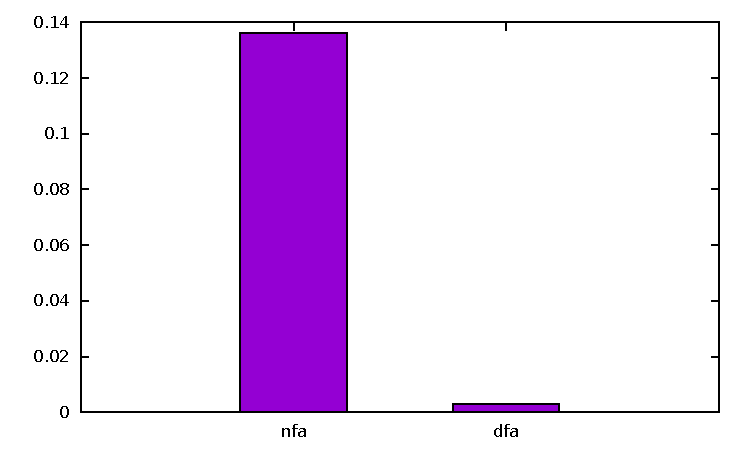
\includegraphics[scale=0.7]{fig/regex.pdf}
	\caption{Benchmark pro knihovnu regex}
    \label{fig:regex}
\end{figure}

Velikost datových struktur pro jednotlivé stavy konečného automatu pro deterministický a nedeterministický
automat je znázorněna v tabulce \ref{tab:regex-size}.

\begin{table}[!htbp]
    \center
    \begin{tabular}{|l|l|}
    \hline
    Typ automatu & Velikost stavu\\ \hhline{|=|=|}
    deterministický  & 24\\ \hline
    nedeterministický & 40\\ \hline
    \end{tabular}
    \caption{Velikosti stavů konečného automatu}
    \label{tab:regex-size}
\end{table}

\chapter{Závěr}\label{chapter:conclusion} % ########################################################################
Cílem této práce bylo popsat a navrhnout aplikační programové rozhraní časově kritických operací využívaných v oblasti
počítačových sítí.
Teoretické základy, ze kterých tato práce vychází, jsou rozvedeny v kapitole \ref{chapter:theoretical}.
Mezi vybrané časově kritické operace patří klasifikace paketů a speciálně pak jednodimenzionální klasifikace paketů
dle cílové IP adresy, hledání nejdelšího shodného prefixu. Pro tuto operaci jsou popsány
algoritmy binárního vyhledávání na délce prefixu a TreeBitmap.
Mezi další rozvedené operace patří hledání řetězců a pro tuto operaci je popsán
algoritmus autorů Aho a Corasickové. Další z operací je hledání regulárních výrazů
za použití konečných automatů, konkrétně deterministického a nedeterministického.
Poslední popsanou operací je analýza a extrakce hlaviček.
Pro každou popsanou operace je navrženo API popsané v kapitole \ref{chapter:api}.

V kapitole \ref{chapter:results} jsou diskutovány výsledky dosažené
při implementaci operací hledání nejdelšího shodného prefixu, hledání řetězců a hledání regulárních
výrazů. Pro hledání nejdelšího shodného prefixu vychází jako nejrychlejší implementace algoritmu
TreeBitmap s velikostí střídy 5. Tohoto výsledku bylo dosaženo na několika datových sadách,
jež vycházejí ze směrovacích tabulek reálný směrovačů.
Pro operaci hledání řetězců bylo experimentování prováděno na síťovém provozu zachyceném
při komunikaci osobního počítače. Jako vzorek
testovaných klíčových slov bylo využito klíčových slov definovaných pro HTTP\footnote{Hyper-text transfer protocol}.
Při experimentování s regulárními výrazy byly jako vstupní data použita stejná data jako pro hledání řetězců,
a jako regulární výrazy byly použity takové regulární výrazy, které dokáží identifikovat URL\footnote{Uniform resource locator} adresu a stavový kód HTTP protokolu.

Jako kroky navazující na tuto práci je možné implementovat zbývající operace, pro které bylo navrženo API ale nebyla provedena implementace. Těmito operacemi je klasifikace paketů a analýza a extrakce hlaviček paketů.

Ze specifikace požadavků na implementaci knihovny v nízkoúrovňovém jazyce C je zřejmé,
že knihovna bude používána i na vestavěných systémech disponujících omezenou pamětí a z toho
důvodu by jedním z dalších kroků mohlo být testování s omezenou operační pamětí.
Je nutné ověřit, že knihovna bude reagovat správným způsobem na nedostatek paměti a nezpůsobí pád systému,
v rámci kterého je spouštěna.

Jedním z dalších možných rozšíření je návrh API a poté implementace vláknového zpracování, které bude
umožňovat zřetězené zpracování jednotlivých operací.
 % viz. obsah.tex

  % Pouzita literatura
  % ----------------------------------------------
\ifczech
  \bibliographystyle{czechiso}
\else
  \bibliographystyle{plain}
%  \bibliographystyle{alpha}
\fi
  \begin{flushleft}
  \bibliography{literatura} % viz. literatura.bib
  \end{flushleft}
  \appendix

  %\chapter{Obsah CD}
%\chapter{Manual}
%\chapter{Konfigrační soubor}
%\chapter{RelaxNG Schéma konfiguračního soboru}
%\chapter{Plakat}

 % viz. prilohy.tex
\end{document}
